\chapter{Utrecht Haskell Compiler}
The type inference system in this thesis is implemented using parts of the Utrecht Haskell compiler. The UHC compiler is a set of different compilers. Its modularity makes it perfect for experimentation.
\section{Design}
The UHC pipeline looks like:
\begin{figure}[H]
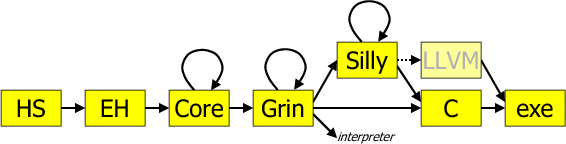
\includegraphics[scale=0.8]{ehc-dataflow2}
\caption{UHC pipeline}
\label{flow}
\end{figure}

For this thesis only the first two phases are interesting. The HS and the EH phases, which are reused:
\begin{description}
\item[\textbf{HS}] In this phase the concrete Haskell syntax is parsed into the abstract syntax. 
\item[\textbf{EH}] The Haskell syntax contains a lot of syntactic sugar. In the EH phase the abstract syntax is desugared and preprocessed.
\end{description}
\subsection{Variant}
UHC as indicated before is a series of smaller compilers. These different versions of the compiler are called \emph{variants}. A tool called \emph{shuffle} is used to weave these variants together. The variant used in this thesis is variant 8. This variant provides no code generation but does provide a parser, renamer, desugarer and typechecker which we can overwrite.

In terms of \emph{Haskell98} all the needed constructs are there except for \emph{type classes}. This variant is simple enough to be implemented in the alloted time, but complete enough that we can implement a large subset of Haskell functionality using it. Including higher-rank functions.

\subsection{EH}
The abstract language used by the Utrecht Haskell Compiler (UHC) to represent desugared Haskell is called Essential Haskell or EH for short. EH at its core resembles $\lambda-calculus$ but with added \textbf{Let} bindings. EH denotes a Haskell file but with all the syntactical sugar of the HS file removed, leaving only a core set of basic operations that need to be supported.
